\documentclass{article}
\usepackage{tikz}
\begin{document}
\begin{huge}
$$C_{3v}$$
and also
$$D_{3h}$$
\end{huge}
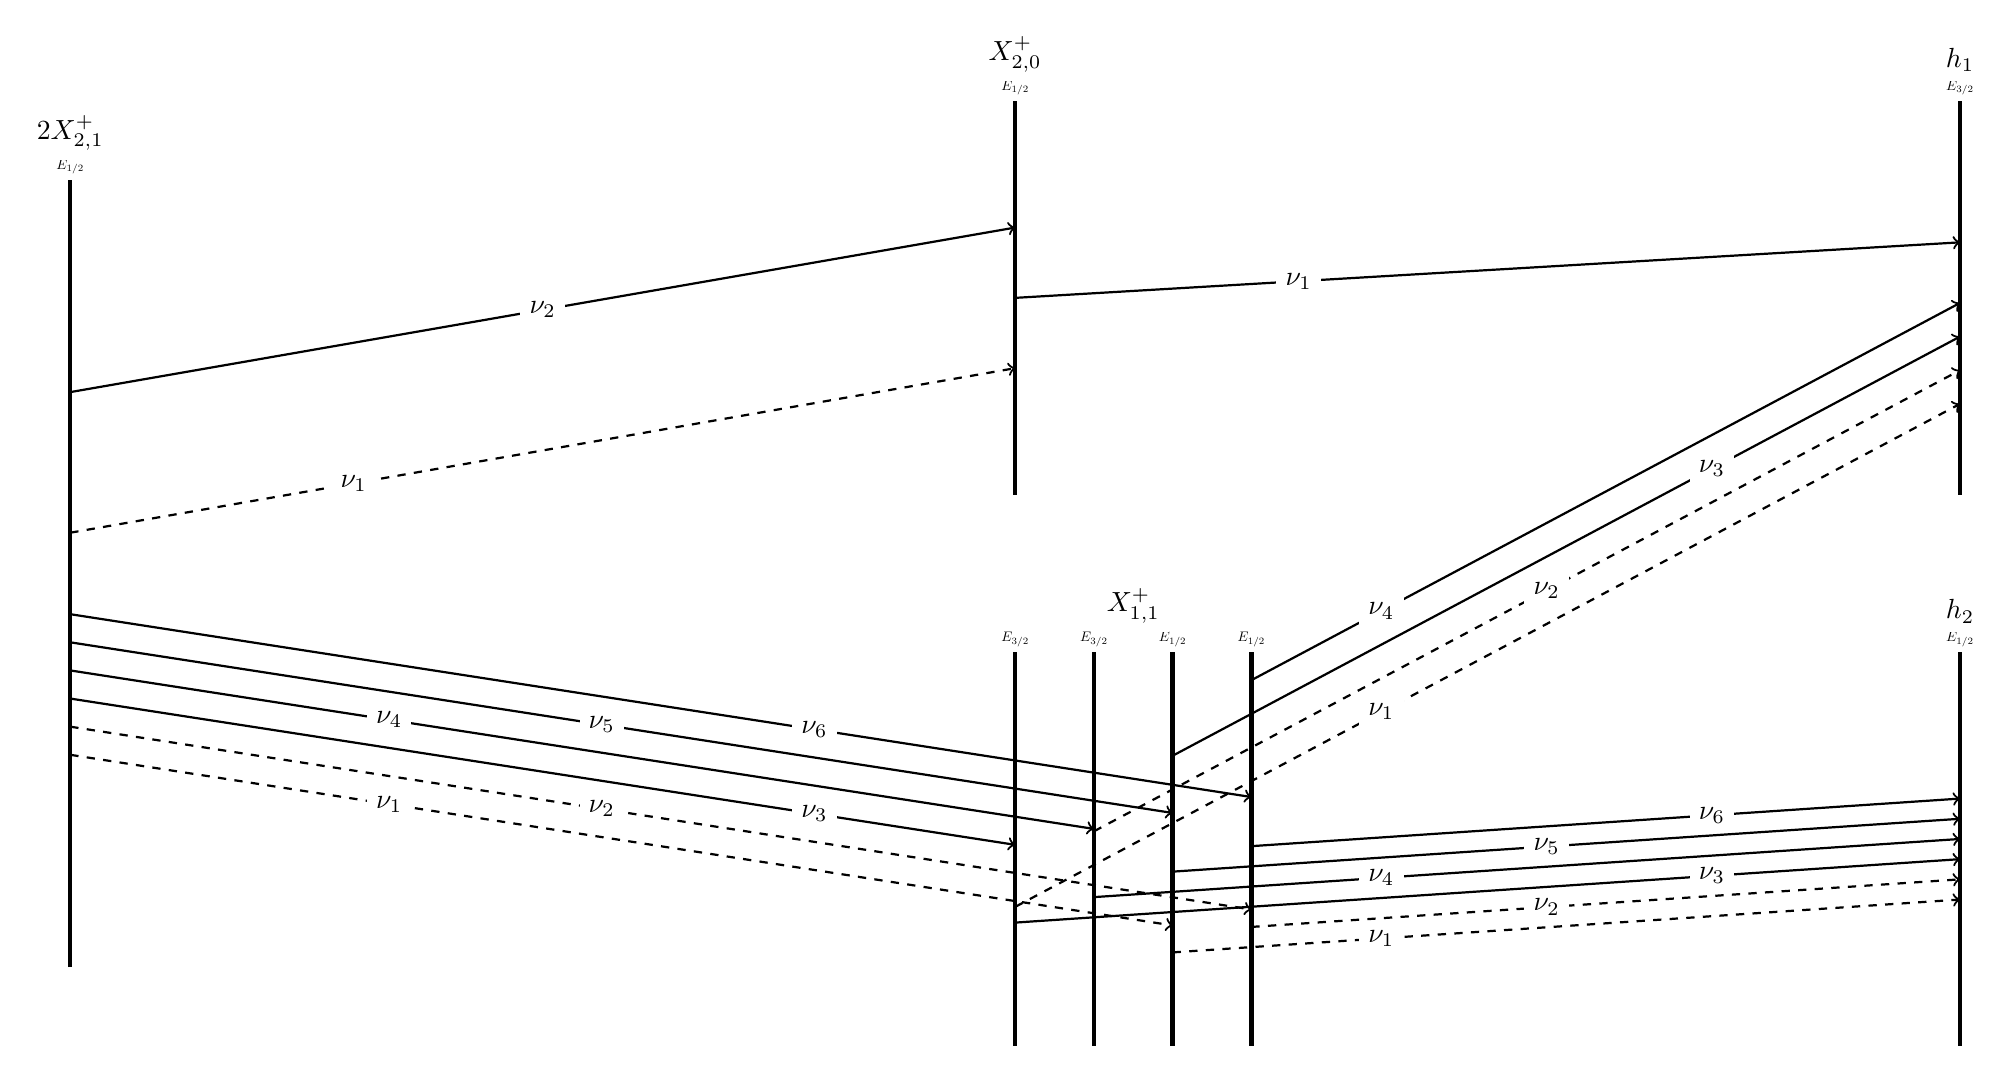
\begin{tikzpicture}[scale=1]
\draw[ultra thick] (-5,-1.5) -- (-5,8.5) node[above=0pt,fill=white,pos=1.0,scale=0.5] {$E_{1/2}$};
\path (-5,8.5) -- (-5,8.5) node[above=7pt,fill=white,pos=0.5,scale=1] {$2X_{2,1}^+$};
\draw[ultra thick] (7,-2.5) -- (7,2.5) node[above=0pt,fill=white,pos=1.0,scale=0.5] {$E_{3/2}$};
\draw[ultra thick] (8,-2.5) -- (8,2.5) node[above=0pt,fill=white,pos=1.0,scale=0.5] {$E_{3/2}$};
\draw[ultra thick] (9,-2.5) -- (9,2.5) node[above=0pt,fill=white,pos=1.0,scale=0.5] {$E_{1/2}$};
\draw[ultra thick] (10,-2.5) -- (10,2.5) node[above=0pt,fill=white,pos=1.0,scale=0.5] {$E_{1/2}$};
\path (7,2.5) -- (10,2.5) node[above=7pt,fill=white,pos=0.5,scale=1] {$X_{1,1}^+$};
\draw[ultra thick] (7,4.5) -- (7,9.5) node[above=0pt,fill=white,pos=1.0,scale=0.5] {$E_{1/2}$};
\path (7,9.5) -- (7,9.5) node[above=7pt,fill=white,pos=0.5,scale=1] {$X_{2,0}^+$};
\draw[ultra thick] (19,-2.5) -- (19,2.5) node[above=0pt,fill=white,pos=1.0,scale=0.5] {$E_{1/2}$};
\path (19,2.5) -- (19,2.5) node[above=7pt,fill=white,pos=0.5,scale=1] {$h_2$};
\draw[ultra thick] (19,4.5) -- (19,9.5) node[above=0pt,fill=white,pos=1.0,scale=0.5] {$E_{3/2}$};
\path (19,9.5) -- (19,9.5) node[above=7pt,fill=white,pos=0.5,scale=1] {$h_1$};
\draw[dashed,->,thick] (-5,1.19689) -- (9,-0.97026);
\path (-5,1.19689) -- (8.5,-0.89286) node[fill=white,pos=0.3] {$\nu_1$};
\draw[dashed,->,thick] (-5,1.55403) -- (10,-0.76791);
\path (-5,1.55403) -- (8.5,-0.53571) node[fill=white,pos=0.5] {$\nu_2$};
\draw[solid,->,thick] (-5,1.91117) -- (7,0.05362);
\path (-5,1.91117) -- (8.5,-0.17857) node[fill=white,pos=0.7] {$\nu_3$};
\draw[solid,->,thick] (-5,2.26832) -- (8,0.25597);
\path (-5,2.26832) -- (8.5,0.17857) node[fill=white,pos=0.3] {$\nu_4$};
\draw[solid,->,thick] (-5,2.62546) -- (9,0.45832);
\path (-5,2.62546) -- (8.5,0.53571) node[fill=white,pos=0.5] {$\nu_5$};
\draw[solid,->,thick] (-5,2.9826) -- (10,0.66066);
\path (-5,2.9826) -- (8.5,0.89286) node[fill=white,pos=0.7] {$\nu_6$};
\draw[dashed,->,thick] (-5,4.0174) -- (7,6.10714);
\path (-5,4.0174) -- (7,6.10714) node[fill=white,pos=0.3] {$\nu_1$};
\draw[solid,->,thick] (-5,5.80311) -- (7,7.89286);
\path (-5,5.80311) -- (7,7.89286) node[fill=white,pos=0.5] {$\nu_2$};
\draw[dashed,->,thick] (9,-1.31258) -- (19,-0.64103);
\path (8.5,-1.34615) -- (19,-0.64103) node[fill=white,pos=0.3] {$\nu_1$};
\draw[dashed,->,thick] (10,-0.98901) -- (19,-0.38462);
\path (8.5,-1.08974) -- (19,-0.38462) node[fill=white,pos=0.5] {$\nu_2$};
\draw[solid,->,thick] (7,-0.93407) -- (19,-0.12821);
\path (8.5,-0.83333) -- (19,-0.12821) node[fill=white,pos=0.7] {$\nu_3$};
\draw[solid,->,thick] (8,-0.6105) -- (19,0.12821);
\path (8.5,-0.57692) -- (19,0.12821) node[fill=white,pos=0.3] {$\nu_4$};
\draw[solid,->,thick] (9,-0.28694) -- (19,0.38462);
\path (8.5,-0.32051) -- (19,0.38462) node[fill=white,pos=0.5] {$\nu_5$};
\draw[solid,->,thick] (10,0.03663) -- (19,0.64103);
\path (8.5,-0.0641) -- (19,0.64103) node[fill=white,pos=0.7] {$\nu_6$};
\draw[dashed,->,thick] (7,-0.73443) -- (19,5.65385);
\path (8.5,0.0641) -- (19,5.65385) node[fill=white,pos=0.3] {$\nu_1$};
\draw[dashed,->,thick] (8,0.22527) -- (19,6.0812);
\path (8.5,0.49145) -- (19,6.0812) node[fill=white,pos=0.5] {$\nu_2$};
\draw[solid,->,thick] (9,1.18498) -- (19,6.50855);
\path (8.5,0.9188) -- (19,6.50855) node[fill=white,pos=0.7] {$\nu_3$};
\draw[solid,->,thick] (10,2.14469) -- (19,6.9359);
\path (8.5,1.34615) -- (19,6.9359) node[fill=white,pos=0.3] {$\nu_4$};
\draw[solid,->,thick] (7,7) -- (19,7.70513);
\path (7,7) -- (19,7.70513) node[fill=white,pos=0.3] {$\nu_1$};
\end{tikzpicture}
\end{document}